%%%%%%%%%%%%%%%%%%%%%%%%%%%%%%%%%%%%%%%%%
% Memo
% LaTeX Template
% Version 1.0 (30/12/13)
%
% This template has been downloaded from:
% http://www.LaTeXTemplates.com
%
% Original author:
% Rob Oakes (http://www.oak-tree.us) with modifications by:
% Vel (vel@latextemplates.com)
%
% License:
% CC BY-NC-SA 3.0 (http://creativecommons.org/licenses/by-nc-sa/3.0/)
%

\documentclass[letterpaper,11pt]{texMemo} % Set the paper size (letterpaper, a4paper, etc) and font size (10pt, 11pt or 12pt)

\usepackage{parskip} % Adds spacing between paragraphs
\usepackage[colorlinks]{hyperref}
\usepackage{graphicx}
\usepackage{float}
\usepackage{hyperref}
\usepackage{listings}
\hypersetup{citecolor=DeepPink4}
\hypersetup{linkcolor=red}
\hypersetup{urlcolor=blue}
\usepackage{cleveref}
\setlength{\parindent}{15pt} % Indent paragraphs

%----------------------------------------------------------------------------------------
%	MEMO INFORMATION
%----------------------------------------------------------------------------------------

\memoto{Dr.Randy Hoover} % Recipient(s)

\memofrom{Benjamin LeBrun, Benjamin Garcia} % Sender(s)

\memosubject{Final Lab Assignment: Autonomous/Semi-Autonomous robots } % Memo subject

\memodate{\today} % Date, set to \today for automatically printing todays date

%----------------------------------------------------------------------------------------

\begin{document}

\maketitle % Print the memo header information

%----------------------------------------------------------------------------------------
%	MEMO CONTENT
%----------------------------------------------------------------------------------------

\section*{Introduction}
For this lab, we utilized the entire robot kit to traverse through a 
maze autonomously using the ultrasonic distance sensor and the line
followers on the bottom of the robot. Then, we utilize a computer as a
middleware between a game controller and the robot over bluetooth to send 
instructions wirelessly to attempt to move blocks on a playing field.

\section*{Equipment}
The primary devices we used were:

\begin{itemize}
    \item Acrylic vehicle body with screws, assembled
    \item Elegoo Uno (chip: Atmega328p)
    \item HC-SR04 ultrasonic distance sensor
    \item SG 90 hobby servo motor
    \item ZS - 040 Bluetooth sensor
    \item Tri-line sensor
    \item 4 DC motors
    \item L298 motor controller
    \item Dualshock 4 controller
    \item 2 ICR18650 batteries with battery box
    \item Ribbon cables
    \item Host laptop with AVR-gcc 8-bit toolchain
    \item USB 2.0 A to B cable
    \item (optional) Logitech G29 sim racing wheel
\end{itemize}

\subsection*{Configuration}
Our robot vehicle was assembled according to Elegoo's instructions which can be found
on Elegoo's website at \url{https://www.elegoo.com/download/}. For this lab, we are
using the V3.0 version of the robot kit.

Using the cumulative code we wrote throughout the semester, we combined all components and 
their corresponding operational code to attempt to drive the robot autonomously through a maze.
After a 30 second timer expires or we cross a taped line on the course, we then will turn 
to manual control mode. Here we used code in Python to act as a middleware between the robot and 
a Dualshock 4 controller, utilizing the joysticks as wheel controls for direction forwards and back 
and also speed control based on the stick's forward and back position. These are serialized and sent over
uart to the robot to interpret and drive the motors.

\begin{figure}[!ht]
\begin{center}
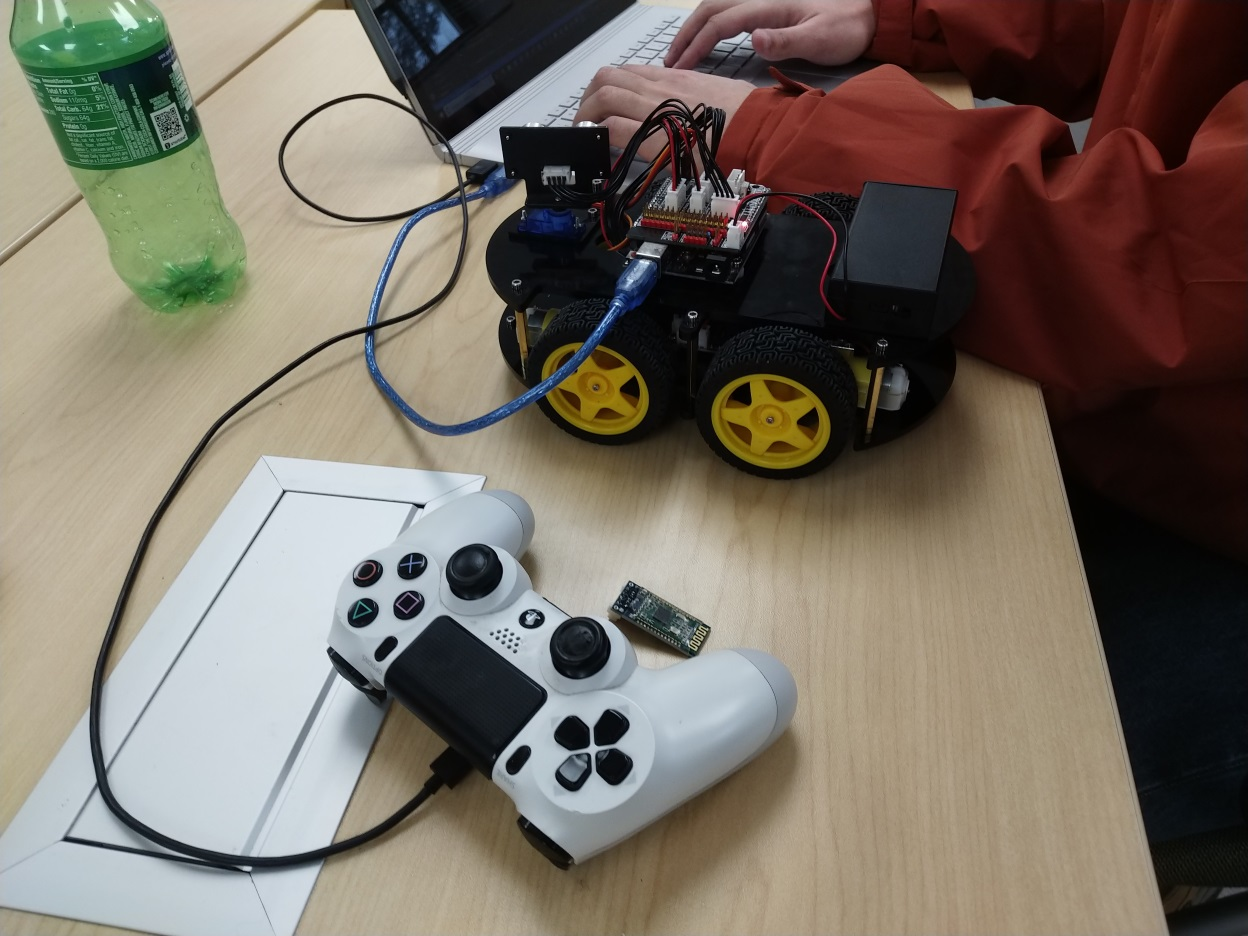
\includegraphics[width=\linewidth]{robot.jpg}
\end{center}
\caption{Servo with ultrasonic sensor assembly.}
\label{fig:f4}
\end{figure}

\section*{Implementation}
For this lab we are using previously written abstraction functions inside of an 
ai.c and ai.h files which were designed to be implemented as individual code
sections for top level implementation of all of our devices. This allows us 
to efficiently write the autonomy code and the manual control code with minimally
having to revisit previous device code.

In python, we utilize a script that uses the Pygame library to find the controller 
connected to our PC, then use the inputs on the controller to create relative speeds 
to the angle that the sticks are pushed forwards and back on the controller. These 
are then sent with the bleak package over bluetooth from the host computer to the 
robot.

\section*{Discussion}
The very first issue was setting up the controller. Pygame is a tricky piece of code 
that utilizes various event loops and game loops that had to undergo some amount 
of finessing to implement into solid control data and sent to the robot. The data 
received from the controller also had to be processed into speed and direction data, 
all asynchronous as required by the bleak package. We learned that simple is best, 
and attempting to implement complex event loops and individual threads for controller 
motion is a daunting task that we had little time to learn quickly. For this we 
simply check if the controller has a new event every program loop and will attempt 
to extract data from the controller if so. Otherwise, we use previously written data 
in our package.

The next issue is communication. Right now the robot simply cycles through each UART
packet received individually. Our communication backend sends every piece of data 
individually as a single burst, then will relatively assign each received value to 
the pattern of data received on the robot end. This would end with sometimes 
wheel instructions crossing over each other. This was fixed by delimiting the start of every packet with a newline.

Finally, because of the low accuracy of our servo, we had to undergo a number of iterations 
through our autonomy code. First we tried absolute distance judgment from each of the turns 
of the servo and ultrasonic ping. Sometimes junk data would be produced, as when the servo 
didn't make a full 90 degree turn or measured a distance that was incorrect 
to the robot's left or right. We fixed this by adding very long delays between sensor readings and performing only one reading at a time, rather than gathering all of the distances across the arc of the servo. We made this work by making the robot move a larger distance in each decision pass, and by having the robot prefer the most likely motions in a priority order, thus requiring fewer sensor reads.

%TODO GAMEDAY PERFORMANCE

%TODO ADDITIONAL ENHANCEMENTS
 

\newpage
\section*{Appendices}
Table of contents:
\begin{itemize}
    \item ai.h - Autonomy code header
    \item ai.c - Main autonomy code, controls motors and readings
    \item main.c - entry, initialization and drive instructions
    \item bit\_macros.h - bit manipulations macros
    \item globals.h - global variables needed by libraries using timers
    \item pcint.h - Pin change interrupt header for ultrasonic sensor
    \item pcint.c - Pin change interrupt code for ultrasonic sensor
    \item pin\_map.h - Pin map header for device
    \item robotio.h - UART control header
    \item robotio.c - UART control code
    \item servo.h - Servo control library
    \item servo.c - Servo control code
    \item timers.h - Timers control library
    \item timers.c - Timers control code
    \item ultrasonic.h - Ultrasonic header file
    \item ultrasonic.c - Ultrasonic code file
\end{itemize}
\newpage

\section*{Appendix A: ai.h}
\begin{tiny}
\lstinputlisting{../ai.h}
\end{tiny}
\newpage

\section*{Appendix B: ai.c}
\begin{tiny}
\lstinputlisting{../ai.c}
\end{tiny}
\newpage

\section*{Appendix C: main.c}
\begin{tiny}
\lstinputlisting{../main.c}
\end{tiny}
\newpage

\section*{Appendix D: bit\_macros.h}
\begin{tiny}
\lstinputlisting{../bit_macros.h}
\end{tiny}
\newpage

\section*{Appendix E: globals.h}
\begin{tiny}
\lstinputlisting{../globals.h}
\end{tiny}
\newpage

\section*{Appendix F: pcint.h}
\begin{tiny}
\lstinputlisting{../pcint.c}
\end{tiny}
\newpage

\section*{Appendix G: pcint.c}
\begin{tiny}
\lstinputlisting{../pcint.c}
\end{tiny}
\newpage

\section*{Appendix H: pin\_map.h}
\begin{tiny}
\lstinputlisting{../pin_map.h}
\end{tiny}
\newpage

\section*{Appendix I: robotio.h}
\begin{tiny}
\lstinputlisting{../robotio.h}
\end{tiny}
\newpage

\section*{Appendix J: robotio.c}
\begin{tiny}
\lstinputlisting{../robotio.c}
\end{tiny}
\newpage

\section*{Appendix K: servo.h}
\begin{tiny}
\lstinputlisting{../servo.h}
\end{tiny}
\newpage

\section*{Appendix L: servo.c}
\begin{tiny}
\lstinputlisting{../servo.c}
\end{tiny}
\newpage

\section*{Appendix M: timers.h}
\begin{tiny}
\lstinputlisting{../timers.h}
\end{tiny}
\newpage

\section*{Appendix N: timers.c}
\begin{tiny}
\lstinputlisting{../timers.c}
\end{tiny}
\newpage

\section*{Appendix O: ultrasonic.h}
\begin{tiny}
\lstinputlisting{../ultrasonic.h}
\end{tiny}
\newpage

\section*{Appendix P: ultrasonic.c}
\begin{tiny}
\lstinputlisting{../ultrasonic.c}
\end{tiny}
\newpage

\end{document}
\grid
